\documentclass[twoside]{book}

% Packages required by doxygen
\usepackage{fixltx2e}
\usepackage{calc}
\usepackage{doxygen}
\usepackage[export]{adjustbox} % also loads graphicx
\usepackage{graphicx}
\usepackage[utf8]{inputenc}
\usepackage{makeidx}
\usepackage{multicol}
\usepackage{multirow}
\PassOptionsToPackage{warn}{textcomp}
\usepackage{textcomp}
\usepackage[nointegrals]{wasysym}
\usepackage[table]{xcolor}

% Font selection
\usepackage[T1]{fontenc}
\usepackage[scaled=.90]{helvet}
\usepackage{courier}
\usepackage{amssymb}
\usepackage{sectsty}
\renewcommand{\familydefault}{\sfdefault}
\allsectionsfont{%
  \fontseries{bc}\selectfont%
  \color{darkgray}%
}
\renewcommand{\DoxyLabelFont}{%
  \fontseries{bc}\selectfont%
  \color{darkgray}%
}
\newcommand{\+}{\discretionary{\mbox{\scriptsize$\hookleftarrow$}}{}{}}

% Page & text layout
\usepackage{geometry}
\geometry{%
  a4paper,%
  top=2.5cm,%
  bottom=2.5cm,%
  left=2.5cm,%
  right=2.5cm%
}
\tolerance=750
\hfuzz=15pt
\hbadness=750
\setlength{\emergencystretch}{15pt}
\setlength{\parindent}{0cm}
\setlength{\parskip}{3ex plus 2ex minus 2ex}
\makeatletter
\renewcommand{\paragraph}{%
  \@startsection{paragraph}{4}{0ex}{-1.0ex}{1.0ex}{%
    \normalfont\normalsize\bfseries\SS@parafont%
  }%
}
\renewcommand{\subparagraph}{%
  \@startsection{subparagraph}{5}{0ex}{-1.0ex}{1.0ex}{%
    \normalfont\normalsize\bfseries\SS@subparafont%
  }%
}
\makeatother

% Headers & footers
\usepackage{fancyhdr}
\pagestyle{fancyplain}
\fancyhead[LE]{\fancyplain{}{\bfseries\thepage}}
\fancyhead[CE]{\fancyplain{}{}}
\fancyhead[RE]{\fancyplain{}{\bfseries\leftmark}}
\fancyhead[LO]{\fancyplain{}{\bfseries\rightmark}}
\fancyhead[CO]{\fancyplain{}{}}
\fancyhead[RO]{\fancyplain{}{\bfseries\thepage}}
\fancyfoot[LE]{\fancyplain{}{}}
\fancyfoot[CE]{\fancyplain{}{}}
\fancyfoot[RE]{\fancyplain{}{\bfseries\scriptsize Generated by Doxygen }}
\fancyfoot[LO]{\fancyplain{}{\bfseries\scriptsize Generated by Doxygen }}
\fancyfoot[CO]{\fancyplain{}{}}
\fancyfoot[RO]{\fancyplain{}{}}
\renewcommand{\footrulewidth}{0.4pt}
\renewcommand{\chaptermark}[1]{%
  \markboth{#1}{}%
}
\renewcommand{\sectionmark}[1]{%
  \markright{\thesection\ #1}%
}

% Indices & bibliography
\usepackage{natbib}
\usepackage[titles]{tocloft}
\setcounter{tocdepth}{3}
\setcounter{secnumdepth}{5}
\makeindex

% Hyperlinks (required, but should be loaded last)
\usepackage{ifpdf}
\ifpdf
  \usepackage[pdftex,pagebackref=true]{hyperref}
\else
  \usepackage[ps2pdf,pagebackref=true]{hyperref}
\fi
\hypersetup{%
  colorlinks=true,%
  linkcolor=blue,%
  citecolor=blue,%
  unicode%
}

% Custom commands
\newcommand{\clearemptydoublepage}{%
  \newpage{\pagestyle{empty}\cleardoublepage}%
}

\usepackage{caption}
\captionsetup{labelsep=space,justification=centering,font={bf},singlelinecheck=off,skip=4pt,position=top}

%===== C O N T E N T S =====

\begin{document}

% Titlepage & ToC
\hypersetup{pageanchor=false,
             bookmarksnumbered=true,
             pdfencoding=unicode
            }
\pagenumbering{roman}
\begin{titlepage}
\vspace*{7cm}
\begin{center}%
{\Large Flip\+\_\+flop }\\
\vspace*{1cm}
{\large Generated by Doxygen 1.8.11}\\
\end{center}
\end{titlepage}
\clearemptydoublepage
\tableofcontents
\clearemptydoublepage
\pagenumbering{arabic}
\hypersetup{pageanchor=true}

%--- Begin generated contents ---
\chapter{Design Unit Index}
\section{Design Unit Hierarchy}
This inheritance list is sorted roughly, but not completely, alphabetically\+:\begin{DoxyCompactList}
\item \contentsline{section}{tb\+\_\+\+Flip\+\_\+flop\+\_\+\+R\+\_\+W}{\pageref{classtb___flip__flop___r___w}}{}
\begin{DoxyCompactList}
\item \contentsline{section}{Flip\+\_\+flop\+\_\+\+R\+\_\+W}{\pageref{class_flip__flop___r___w}}{}
\end{DoxyCompactList}
\item \contentsline{section}{tb\+\_\+\+Flip\+\_\+flop\+\_\+\+R\+C\+\_\+S}{\pageref{classtb___flip__flop___r_c___s}}{}
\begin{DoxyCompactList}
\item \contentsline{section}{Flip\+\_\+flop\+\_\+\+R\+C\+\_\+S}{\pageref{class_flip__flop___r_c___s}}{}
\end{DoxyCompactList}
\end{DoxyCompactList}

\chapter{Design Unit Index}
\section{Design Unit List}
Here is a list of all design unit members with links to the Entities they belong to\+:\begin{DoxyCompactList}
\item\contentsline{section}{architecture \hyperlink{classtb__cascadable__counter_1_1_behavioral}{Behavioral} \\*Architecture definition of the \hyperlink{classtb__cascadable__counter}{tb\+\_\+cascadable\+\_\+counter} }{\pageref{classtb__cascadable__counter_1_1_behavioral}}{}
\item\contentsline{section}{entity \hyperlink{classcascadable__counter}{cascadable\+\_\+counter} }{\pageref{classcascadable__counter}}{}
\item\contentsline{section}{architecture \hyperlink{classcascadable__counter_1_1fsm}{fsm} \\*Architecture definition of the \hyperlink{classcascadable__counter}{cascadable\+\_\+counter} }{\pageref{classcascadable__counter_1_1fsm}}{}
\item\contentsline{section}{entity \hyperlink{classtb__cascadable__counter}{tb\+\_\+cascadable\+\_\+counter} }{\pageref{classtb__cascadable__counter}}{}
\end{DoxyCompactList}

\chapter{File Index}
\section{File List}
Here is a list of all documented files with brief descriptions\+:\begin{DoxyCompactList}
\item\contentsline{section}{C\+:/\+Users/\+Public/\+Documents/\+Github/\+V\+H\+D\+L/\+Flip\+\_\+flop/\hyperlink{_flip__flop___r___w_8vhd}{Flip\+\_\+flop\+\_\+\+R\+\_\+\+W.\+vhd} \\*\hyperlink{class_flip__flop___r___w}{Flip\+\_\+flop\+\_\+\+R\+\_\+W} \+: This entity with synchronization reset is uesd to perform a special port. It could be read by microcontroller and writen by I2C. That means if I2C set \textquotesingle{}i2c\+\_\+write\textquotesingle{} on one, it would put the data of \textquotesingle{}i2c\+\_\+data\+\_\+in\textquotesingle{} into the output \textquotesingle{}uc\+\_\+read\textquotesingle{}. It could be one or zero.\+It just likes its write fonction. Then we can use its output as the input of microcontroller. It likes read by microcontroller }{\pageref{_flip__flop___r___w_8vhd}}{}
\item\contentsline{section}{C\+:/\+Users/\+Public/\+Documents/\+Github/\+V\+H\+D\+L/\+Flip\+\_\+flop/\hyperlink{_flip__flop___r_c___s_8vhd}{Flip\+\_\+flop\+\_\+\+R\+C\+\_\+\+S.\+vhd} \\*\hyperlink{class_flip__flop___r_c___s}{Flip\+\_\+flop\+\_\+\+R\+C\+\_\+S} \+: This entity with synchronization reset is uesd to perform a special port. It could be read or cleared by microcontroller and writen by I2C. That means if microcontroller set \textquotesingle{}uc\+\_\+clear\textquotesingle{} on one, it would set the output on zero. If I2C set \textquotesingle{}i2c\+\_\+set\textquotesingle{} on one, it would set the output on one. It just likes its set fonction. Then we can use its output as the input of microcontroller. It likes read by microcontroller }{\pageref{_flip__flop___r_c___s_8vhd}}{}
\item\contentsline{section}{C\+:/\+Users/\+Public/\+Documents/\+Github/\+V\+H\+D\+L/\+Flip\+\_\+flop/\hyperlink{tb___flip__flop___r___w_8vhd}{tb\+\_\+\+Flip\+\_\+flop\+\_\+\+R\+\_\+\+W.\+vhd} \\*Tb\+\_\+\+Flip\+\_\+flop\+\_\+\+R\+\_\+W \+:testbench for the entity flip\+\_\+flop\+\_\+r\+\_\+w }{\pageref{tb___flip__flop___r___w_8vhd}}{}
\item\contentsline{section}{C\+:/\+Users/\+Public/\+Documents/\+Github/\+V\+H\+D\+L/\+Flip\+\_\+flop/\hyperlink{tb___flip__flop___r_c___s_8vhd}{tb\+\_\+\+Flip\+\_\+flop\+\_\+\+R\+C\+\_\+\+S.\+vhd} \\*Tb\+\_\+\+Flip\+\_\+flop\+\_\+\+R\+C\+\_\+S \+:testbench for the entity flip\+\_\+flop\+\_\+rc\+\_\+s }{\pageref{tb___flip__flop___r_c___s_8vhd}}{}
\end{DoxyCompactList}

\chapter{Class Documentation}
\hypertarget{class_flip__flop___r___w_1_1_behavioral}{}\section{Behavioral Architecture Reference}
\label{class_flip__flop___r___w_1_1_behavioral}\index{Behavioral@{Behavioral}}


Architecture definition of the \hyperlink{class_flip__flop___r___w}{Flip\+\_\+flop\+\_\+\+R\+\_\+W}.  


\subsection*{Processes}
 \begin{DoxyCompactItemize}
\item 
\hyperlink{class_flip__flop___r___w_1_1_behavioral_afacea8133ab3b379b47608b352cd8766}{combination}{\bfseries  ( {\bfseries \textcolor{vhdlchar}{clk}\textcolor{vhdlchar}{ }} )}
\begin{DoxyCompactList}\small\item\em Process combination of the Architecture. \end{DoxyCompactList}\end{DoxyCompactItemize}


\subsection{Detailed Description}
Architecture definition of the \hyperlink{class_flip__flop___r___w}{Flip\+\_\+flop\+\_\+\+R\+\_\+W}. 

More details about this \hyperlink{class_flip__flop___r___w}{Flip\+\_\+flop\+\_\+\+R\+\_\+W} element. 

\subsection{Member Function Documentation}
\index{Flip\+\_\+flop\+\_\+\+R\+\_\+\+W\+::\+Behavioral@{Flip\+\_\+flop\+\_\+\+R\+\_\+\+W\+::\+Behavioral}!combination@{combination}}
\index{combination@{combination}!Flip\+\_\+flop\+\_\+\+R\+\_\+\+W\+::\+Behavioral@{Flip\+\_\+flop\+\_\+\+R\+\_\+\+W\+::\+Behavioral}}
\subsubsection[{\texorpdfstring{combinationclk}{combinationclk}}]{\setlength{\rightskip}{0pt plus 5cm} {\bfseries \textcolor{vhdlchar}{ }} combination(
\begin{DoxyParamCaption}
\item[{}]{{\bfseries \textcolor{vhdlchar}{clk}\textcolor{vhdlchar}{ }} {\em }}
\end{DoxyParamCaption}
)\hspace{0.3cm}{\ttfamily [Process]}}\hypertarget{class_flip__flop___r___w_1_1_behavioral_afacea8133ab3b379b47608b352cd8766}{}\label{class_flip__flop___r___w_1_1_behavioral_afacea8133ab3b379b47608b352cd8766}


Process combination of the Architecture. 

More details about this combination element. 

The documentation for this class was generated from the following file\+:\begin{DoxyCompactItemize}
\item 
C\+:/\+Users/\+Public/\+Documents/\+Github/\+V\+H\+D\+L/\+Flip\+\_\+flop/\hyperlink{_flip__flop___r___w_8vhd}{Flip\+\_\+flop\+\_\+\+R\+\_\+\+W.\+vhd}\end{DoxyCompactItemize}

\hypertarget{class_flip__flop___r_c___s_1_1_behavioral}{}\section{Behavioral Architecture Reference}
\label{class_flip__flop___r_c___s_1_1_behavioral}\index{Behavioral@{Behavioral}}


Architecture definition of the \hyperlink{class_flip__flop___r_c___s}{Flip\+\_\+flop\+\_\+\+R\+C\+\_\+S}.  


\subsection*{Processes}
 \begin{DoxyCompactItemize}
\item 
\hyperlink{class_flip__flop___r_c___s_1_1_behavioral_afacea8133ab3b379b47608b352cd8766}{combination}{\bfseries  ( {\bfseries \textcolor{vhdlchar}{clk}\textcolor{vhdlchar}{ }} )}
\begin{DoxyCompactList}\small\item\em Process combination of the Architecture. \end{DoxyCompactList}\end{DoxyCompactItemize}


\subsection{Detailed Description}
Architecture definition of the \hyperlink{class_flip__flop___r_c___s}{Flip\+\_\+flop\+\_\+\+R\+C\+\_\+S}. 

More details about this \hyperlink{class_flip__flop___r_c___s}{Flip\+\_\+flop\+\_\+\+R\+C\+\_\+S} element. 

\subsection{Member Function Documentation}
\index{Flip\+\_\+flop\+\_\+\+R\+C\+\_\+\+S\+::\+Behavioral@{Flip\+\_\+flop\+\_\+\+R\+C\+\_\+\+S\+::\+Behavioral}!combination@{combination}}
\index{combination@{combination}!Flip\+\_\+flop\+\_\+\+R\+C\+\_\+\+S\+::\+Behavioral@{Flip\+\_\+flop\+\_\+\+R\+C\+\_\+\+S\+::\+Behavioral}}
\subsubsection[{\texorpdfstring{combinationclk}{combinationclk}}]{\setlength{\rightskip}{0pt plus 5cm} {\bfseries \textcolor{vhdlchar}{ }} combination(
\begin{DoxyParamCaption}
\item[{}]{{\bfseries \textcolor{vhdlchar}{clk}\textcolor{vhdlchar}{ }} {\em }}
\end{DoxyParamCaption}
)\hspace{0.3cm}{\ttfamily [Process]}}\hypertarget{class_flip__flop___r_c___s_1_1_behavioral_afacea8133ab3b379b47608b352cd8766}{}\label{class_flip__flop___r_c___s_1_1_behavioral_afacea8133ab3b379b47608b352cd8766}


Process combination of the Architecture. 

More details about this combination element. 

The documentation for this class was generated from the following file\+:\begin{DoxyCompactItemize}
\item 
C\+:/\+Users/\+Public/\+Documents/\+Github/\+V\+H\+D\+L/\+Flip\+\_\+flop/\hyperlink{_flip__flop___r_c___s_8vhd}{Flip\+\_\+flop\+\_\+\+R\+C\+\_\+\+S.\+vhd}\end{DoxyCompactItemize}

\hypertarget{classtb___flip__flop___r_c___s_1_1_behavioral}{}\section{Behavioral Architecture Reference}
\label{classtb___flip__flop___r_c___s_1_1_behavioral}\index{Behavioral@{Behavioral}}


Architecture definition of the \hyperlink{classtb___flip__flop___r_c___s}{tb\+\_\+\+Flip\+\_\+flop\+\_\+\+R\+C\+\_\+S}.  


\subsection*{Processes}
 \begin{DoxyCompactItemize}
\item 
\hyperlink{classtb___flip__flop___r_c___s_1_1_behavioral_a99f3164d142507cc4972fec85ccfe73a}{clk\+\_\+signal}{\bfseries  (  )}\hypertarget{classtb___flip__flop___r_c___s_1_1_behavioral_a99f3164d142507cc4972fec85ccfe73a}{}\label{classtb___flip__flop___r_c___s_1_1_behavioral_a99f3164d142507cc4972fec85ccfe73a}

\begin{DoxyCompactList}\small\item\em process of generating a clock signal \end{DoxyCompactList}\item 
\hyperlink{classtb___flip__flop___r_c___s_1_1_behavioral_a35fbcf057a197de16f02ae1e198de883}{uc\+\_\+clear\+\_\+signal}{\bfseries  (  )}\hypertarget{classtb___flip__flop___r_c___s_1_1_behavioral_a35fbcf057a197de16f02ae1e198de883}{}\label{classtb___flip__flop___r_c___s_1_1_behavioral_a35fbcf057a197de16f02ae1e198de883}

\begin{DoxyCompactList}\small\item\em process of generating a clear signal by microcontrolleur \end{DoxyCompactList}\item 
\hyperlink{classtb___flip__flop___r_c___s_1_1_behavioral_a35b5be3cd1cb6c47815781e90ca773c6}{i2c\+\_\+set\+\_\+signal}{\bfseries  (  )}\hypertarget{classtb___flip__flop___r_c___s_1_1_behavioral_a35b5be3cd1cb6c47815781e90ca773c6}{}\label{classtb___flip__flop___r_c___s_1_1_behavioral_a35b5be3cd1cb6c47815781e90ca773c6}

\begin{DoxyCompactList}\small\item\em process of generating a set signal by I2C \end{DoxyCompactList}\end{DoxyCompactItemize}
\subsection*{Components}
 \begin{DoxyCompactItemize}
\item 
\hyperlink{classtb___flip__flop___r_c___s_1_1_behavioral_a027f6e762235fee0bc16d610da043d14}{Flip\+\_\+flop\+\_\+\+R\+C\+\_\+S}  {\bfseries }  \hypertarget{classtb___flip__flop___r_c___s_1_1_behavioral_a027f6e762235fee0bc16d610da043d14}{}\label{classtb___flip__flop___r_c___s_1_1_behavioral_a027f6e762235fee0bc16d610da043d14}

\end{DoxyCompactItemize}
\subsection*{Signals}
 \begin{DoxyCompactItemize}
\item 
\hyperlink{classtb___flip__flop___r_c___s_1_1_behavioral_a501952bb7908b845004a8aa030542f7d}{clk} {\bfseries \textcolor{vhdlchar}{S\+T\+D\+\_\+\+L\+O\+G\+IC}\textcolor{vhdlchar}{ }\textcolor{vhdlchar}{ }\textcolor{vhdlchar}{\+:}\textcolor{vhdlchar}{=}\textcolor{vhdlchar}{ }\textcolor{vhdlchar}{ }\textcolor{vhdlchar}{\textquotesingle{}}\textcolor{vhdlchar}{ } \textcolor{vhdldigit}{0} \textcolor{vhdlchar}{ }\textcolor{vhdlchar}{\textquotesingle{}}\textcolor{vhdlchar}{ }} \hypertarget{classtb___flip__flop___r_c___s_1_1_behavioral_a501952bb7908b845004a8aa030542f7d}{}\label{classtb___flip__flop___r_c___s_1_1_behavioral_a501952bb7908b845004a8aa030542f7d}

\begin{DoxyCompactList}\small\item\em use signals internals simulate these ports of component \end{DoxyCompactList}\item 
\hyperlink{classtb___flip__flop___r_c___s_1_1_behavioral_a7e333d8b89f48acd3c4ac58948c1afb8}{clk\+\_\+ena} {\bfseries \textcolor{vhdlchar}{S\+T\+D\+\_\+\+L\+O\+G\+IC}\textcolor{vhdlchar}{ }} \hypertarget{classtb___flip__flop___r_c___s_1_1_behavioral_a7e333d8b89f48acd3c4ac58948c1afb8}{}\label{classtb___flip__flop___r_c___s_1_1_behavioral_a7e333d8b89f48acd3c4ac58948c1afb8}

\item 
\hyperlink{classtb___flip__flop___r_c___s_1_1_behavioral_a5d1d334866b850ea4519655e35c948b9}{sync\+\_\+rst} {\bfseries \textcolor{vhdlchar}{S\+T\+D\+\_\+\+L\+O\+G\+IC}\textcolor{vhdlchar}{ }} \hypertarget{classtb___flip__flop___r_c___s_1_1_behavioral_a5d1d334866b850ea4519655e35c948b9}{}\label{classtb___flip__flop___r_c___s_1_1_behavioral_a5d1d334866b850ea4519655e35c948b9}

\item 
\hyperlink{classtb___flip__flop___r_c___s_1_1_behavioral_a50cf69c237e2cef9a269a0bb7801d630}{uc\+\_\+clear} {\bfseries \textcolor{vhdlchar}{S\+T\+D\+\_\+\+L\+O\+G\+IC}\textcolor{vhdlchar}{ }} \hypertarget{classtb___flip__flop___r_c___s_1_1_behavioral_a50cf69c237e2cef9a269a0bb7801d630}{}\label{classtb___flip__flop___r_c___s_1_1_behavioral_a50cf69c237e2cef9a269a0bb7801d630}

\item 
\hyperlink{classtb___flip__flop___r_c___s_1_1_behavioral_a14a540af3677c9776832614ccbf2416a}{i2c\+\_\+set} {\bfseries \textcolor{vhdlchar}{S\+T\+D\+\_\+\+L\+O\+G\+IC}\textcolor{vhdlchar}{ }} \hypertarget{classtb___flip__flop___r_c___s_1_1_behavioral_a14a540af3677c9776832614ccbf2416a}{}\label{classtb___flip__flop___r_c___s_1_1_behavioral_a14a540af3677c9776832614ccbf2416a}

\item 
\hyperlink{classtb___flip__flop___r_c___s_1_1_behavioral_a190dbf29a2d9cdf803fdac336c49cf66}{uc\+\_\+read} {\bfseries \textcolor{vhdlchar}{S\+T\+D\+\_\+\+L\+O\+G\+IC}\textcolor{vhdlchar}{ }} \hypertarget{classtb___flip__flop___r_c___s_1_1_behavioral_a190dbf29a2d9cdf803fdac336c49cf66}{}\label{classtb___flip__flop___r_c___s_1_1_behavioral_a190dbf29a2d9cdf803fdac336c49cf66}

\end{DoxyCompactItemize}
\subsection*{Instantiations}
 \begin{DoxyCompactItemize}
\item 
\hyperlink{classtb___flip__flop___r_c___s_1_1_behavioral_a1619316ad715601eb5d3559db829ac05}{uut}  {\bfseries Flip\+\_\+flop\+\_\+\+R\+C\+\_\+S}   \hypertarget{classtb___flip__flop___r_c___s_1_1_behavioral_a1619316ad715601eb5d3559db829ac05}{}\label{classtb___flip__flop___r_c___s_1_1_behavioral_a1619316ad715601eb5d3559db829ac05}

\begin{DoxyCompactList}\small\item\em an instance of component \end{DoxyCompactList}\end{DoxyCompactItemize}


\subsection{Detailed Description}
Architecture definition of the \hyperlink{classtb___flip__flop___r_c___s}{tb\+\_\+\+Flip\+\_\+flop\+\_\+\+R\+C\+\_\+S}. 

More details about this \hyperlink{classtb___flip__flop___r_c___s}{tb\+\_\+\+Flip\+\_\+flop\+\_\+\+R\+C\+\_\+S} element. 

The documentation for this class was generated from the following file\+:\begin{DoxyCompactItemize}
\item 
C\+:/\+Users/\+Public/\+Documents/\+Github/\+V\+H\+D\+L/\+Flip\+\_\+flop/\hyperlink{tb___flip__flop___r_c___s_8vhd}{tb\+\_\+\+Flip\+\_\+flop\+\_\+\+R\+C\+\_\+\+S.\+vhd}\end{DoxyCompactItemize}

\hypertarget{classtb___flip__flop___r___w_1_1_behavioral}{}\section{Behavioral Architecture Reference}
\label{classtb___flip__flop___r___w_1_1_behavioral}\index{Behavioral@{Behavioral}}


Architecture definition of the \hyperlink{classtb___flip__flop___r___w}{tb\+\_\+\+Flip\+\_\+flop\+\_\+\+R\+\_\+W}.  


\subsection*{Processes}
 \begin{DoxyCompactItemize}
\item 
\hyperlink{classtb___flip__flop___r___w_1_1_behavioral_a99f3164d142507cc4972fec85ccfe73a}{clk\+\_\+signal}{\bfseries  (  )}\hypertarget{classtb___flip__flop___r___w_1_1_behavioral_a99f3164d142507cc4972fec85ccfe73a}{}\label{classtb___flip__flop___r___w_1_1_behavioral_a99f3164d142507cc4972fec85ccfe73a}

\begin{DoxyCompactList}\small\item\em process of generating a clock signal \end{DoxyCompactList}\item 
\hyperlink{classtb___flip__flop___r___w_1_1_behavioral_a7c5a4e8821909a45cb59f5d44cc12921}{i2c\+\_\+write\+\_\+signal}{\bfseries  (  )}\hypertarget{classtb___flip__flop___r___w_1_1_behavioral_a7c5a4e8821909a45cb59f5d44cc12921}{}\label{classtb___flip__flop___r___w_1_1_behavioral_a7c5a4e8821909a45cb59f5d44cc12921}

\begin{DoxyCompactList}\small\item\em process of generating a write signal by I2C \end{DoxyCompactList}\item 
\hyperlink{classtb___flip__flop___r___w_1_1_behavioral_adb281d3c5a08af1f297d1fa58248de0e}{i2c\+\_\+data\+\_\+in\+\_\+signal}{\bfseries  (  )}\hypertarget{classtb___flip__flop___r___w_1_1_behavioral_adb281d3c5a08af1f297d1fa58248de0e}{}\label{classtb___flip__flop___r___w_1_1_behavioral_adb281d3c5a08af1f297d1fa58248de0e}

\begin{DoxyCompactList}\small\item\em process of generating a data\+\_\+in signal by I2C \end{DoxyCompactList}\end{DoxyCompactItemize}
\subsection*{Components}
 \begin{DoxyCompactItemize}
\item 
\hyperlink{classtb___flip__flop___r___w_1_1_behavioral_a09f8fa8e9617f0d431f9a9cd9c174f60}{Flip\+\_\+flop\+\_\+\+R\+\_\+W}  {\bfseries }  \hypertarget{classtb___flip__flop___r___w_1_1_behavioral_a09f8fa8e9617f0d431f9a9cd9c174f60}{}\label{classtb___flip__flop___r___w_1_1_behavioral_a09f8fa8e9617f0d431f9a9cd9c174f60}

\begin{DoxyCompactList}\small\item\em use a entity as a component \end{DoxyCompactList}\end{DoxyCompactItemize}
\subsection*{Signals}
 \begin{DoxyCompactItemize}
\item 
\hyperlink{classtb___flip__flop___r___w_1_1_behavioral_a501952bb7908b845004a8aa030542f7d}{clk} {\bfseries \textcolor{vhdlchar}{S\+T\+D\+\_\+\+L\+O\+G\+IC}\textcolor{vhdlchar}{ }\textcolor{vhdlchar}{ }\textcolor{vhdlchar}{\+:}\textcolor{vhdlchar}{=}\textcolor{vhdlchar}{ }\textcolor{vhdlchar}{ }\textcolor{vhdlchar}{\textquotesingle{}}\textcolor{vhdlchar}{ } \textcolor{vhdldigit}{0} \textcolor{vhdlchar}{ }\textcolor{vhdlchar}{\textquotesingle{}}\textcolor{vhdlchar}{ }} \hypertarget{classtb___flip__flop___r___w_1_1_behavioral_a501952bb7908b845004a8aa030542f7d}{}\label{classtb___flip__flop___r___w_1_1_behavioral_a501952bb7908b845004a8aa030542f7d}

\begin{DoxyCompactList}\small\item\em use signals internals simulate these ports of component \end{DoxyCompactList}\item 
\hyperlink{classtb___flip__flop___r___w_1_1_behavioral_a7e333d8b89f48acd3c4ac58948c1afb8}{clk\+\_\+ena} {\bfseries \textcolor{vhdlchar}{S\+T\+D\+\_\+\+L\+O\+G\+IC}\textcolor{vhdlchar}{ }} \hypertarget{classtb___flip__flop___r___w_1_1_behavioral_a7e333d8b89f48acd3c4ac58948c1afb8}{}\label{classtb___flip__flop___r___w_1_1_behavioral_a7e333d8b89f48acd3c4ac58948c1afb8}

\item 
\hyperlink{classtb___flip__flop___r___w_1_1_behavioral_a5d1d334866b850ea4519655e35c948b9}{sync\+\_\+rst} {\bfseries \textcolor{vhdlchar}{S\+T\+D\+\_\+\+L\+O\+G\+IC}\textcolor{vhdlchar}{ }} \hypertarget{classtb___flip__flop___r___w_1_1_behavioral_a5d1d334866b850ea4519655e35c948b9}{}\label{classtb___flip__flop___r___w_1_1_behavioral_a5d1d334866b850ea4519655e35c948b9}

\item 
\hyperlink{classtb___flip__flop___r___w_1_1_behavioral_a69317760615591269083e63d8efc021f}{i2c\+\_\+write} {\bfseries \textcolor{vhdlchar}{S\+T\+D\+\_\+\+L\+O\+G\+IC}\textcolor{vhdlchar}{ }} \hypertarget{classtb___flip__flop___r___w_1_1_behavioral_a69317760615591269083e63d8efc021f}{}\label{classtb___flip__flop___r___w_1_1_behavioral_a69317760615591269083e63d8efc021f}

\item 
\hyperlink{classtb___flip__flop___r___w_1_1_behavioral_a3f0f65f93849710f5110c606dbaefccf}{i2c\+\_\+data\+\_\+in} {\bfseries \textcolor{vhdlchar}{S\+T\+D\+\_\+\+L\+O\+G\+IC}\textcolor{vhdlchar}{ }} \hypertarget{classtb___flip__flop___r___w_1_1_behavioral_a3f0f65f93849710f5110c606dbaefccf}{}\label{classtb___flip__flop___r___w_1_1_behavioral_a3f0f65f93849710f5110c606dbaefccf}

\item 
\hyperlink{classtb___flip__flop___r___w_1_1_behavioral_a190dbf29a2d9cdf803fdac336c49cf66}{uc\+\_\+read} {\bfseries \textcolor{vhdlchar}{S\+T\+D\+\_\+\+L\+O\+G\+IC}\textcolor{vhdlchar}{ }} \hypertarget{classtb___flip__flop___r___w_1_1_behavioral_a190dbf29a2d9cdf803fdac336c49cf66}{}\label{classtb___flip__flop___r___w_1_1_behavioral_a190dbf29a2d9cdf803fdac336c49cf66}

\end{DoxyCompactItemize}
\subsection*{Instantiations}
 \begin{DoxyCompactItemize}
\item 
\hyperlink{classtb___flip__flop___r___w_1_1_behavioral_a1619316ad715601eb5d3559db829ac05}{uut}  {\bfseries Flip\+\_\+flop\+\_\+\+R\+\_\+W}   \hypertarget{classtb___flip__flop___r___w_1_1_behavioral_a1619316ad715601eb5d3559db829ac05}{}\label{classtb___flip__flop___r___w_1_1_behavioral_a1619316ad715601eb5d3559db829ac05}

\begin{DoxyCompactList}\small\item\em an instance of component \end{DoxyCompactList}\end{DoxyCompactItemize}


\subsection{Detailed Description}
Architecture definition of the \hyperlink{classtb___flip__flop___r___w}{tb\+\_\+\+Flip\+\_\+flop\+\_\+\+R\+\_\+W}. 

More details about this \hyperlink{classtb___flip__flop___r___w}{tb\+\_\+\+Flip\+\_\+flop\+\_\+\+R\+\_\+W} element. 

The documentation for this class was generated from the following file\+:\begin{DoxyCompactItemize}
\item 
C\+:/\+Users/\+Public/\+Documents/\+Github/\+V\+H\+D\+L/\+Flip\+\_\+flop/\hyperlink{tb___flip__flop___r___w_8vhd}{tb\+\_\+\+Flip\+\_\+flop\+\_\+\+R\+\_\+\+W.\+vhd}\end{DoxyCompactItemize}

\hypertarget{class_flip__flop___r___w}{}\section{Flip\+\_\+flop\+\_\+\+R\+\_\+W Entity Reference}
\label{class_flip__flop___r___w}\index{Flip\+\_\+flop\+\_\+\+R\+\_\+W@{Flip\+\_\+flop\+\_\+\+R\+\_\+W}}
Inheritance diagram for Flip\+\_\+flop\+\_\+\+R\+\_\+W\+:\begin{figure}[H]
\begin{center}
\leavevmode
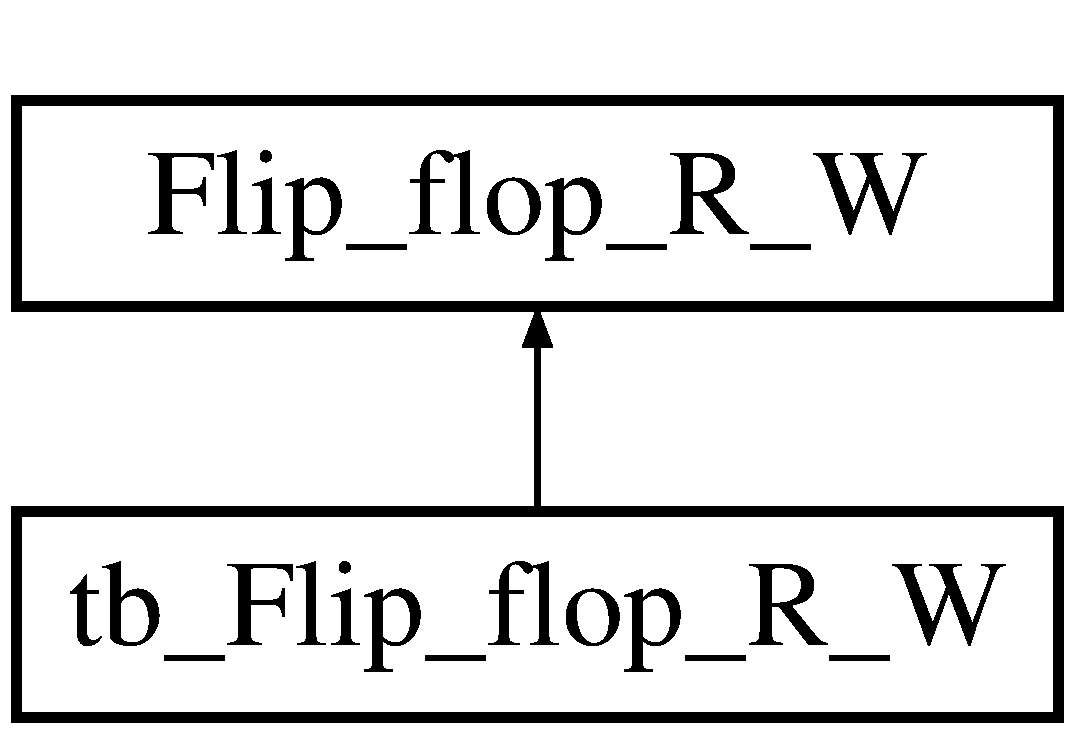
\includegraphics[height=2.000000cm]{class_flip__flop___r___w}
\end{center}
\end{figure}
\subsection*{Entities}
\begin{DoxyCompactItemize}
\item 
\hyperlink{class_flip__flop___r___w_1_1_behavioral}{Behavioral} architecture
\begin{DoxyCompactList}\small\item\em Architecture definition of the \hyperlink{class_flip__flop___r___w}{Flip\+\_\+flop\+\_\+\+R\+\_\+W}. \end{DoxyCompactList}\end{DoxyCompactItemize}
\subsection*{Libraries}
 \begin{DoxyCompactItemize}
\item 
\hyperlink{class_flip__flop___r___w_ae4f03c286607f3181e16b9aa12d0c6d4}{I\+E\+EE} \hypertarget{class_flip__flop___r___w_ae4f03c286607f3181e16b9aa12d0c6d4}{}\label{class_flip__flop___r___w_ae4f03c286607f3181e16b9aa12d0c6d4}

\begin{DoxyCompactList}\small\item\em Use standard library. \end{DoxyCompactList}\end{DoxyCompactItemize}
\subsection*{Use Clauses}
 \begin{DoxyCompactItemize}
\item 
\hyperlink{class_flip__flop___r___w_aa4b2b25246a821511120e3149b003563}{S\+T\+D\+\_\+\+L\+O\+G\+I\+C\+\_\+1164}   \hypertarget{class_flip__flop___r___w_aa4b2b25246a821511120e3149b003563}{}\label{class_flip__flop___r___w_aa4b2b25246a821511120e3149b003563}

\begin{DoxyCompactList}\small\item\em Use logic elements. \end{DoxyCompactList}\end{DoxyCompactItemize}
\subsection*{Ports}
 \begin{DoxyCompactItemize}
\item 
\hyperlink{class_flip__flop___r___w_a6231b307b7958b6060563aa2a93d345a}{clk}  {\bfseries {\bfseries \textcolor{vhdlchar}{in}\textcolor{vhdlchar}{ }}} {\bfseries \textcolor{vhdlchar}{S\+T\+D\+\_\+\+L\+O\+G\+IC}\textcolor{vhdlchar}{ }} \hypertarget{class_flip__flop___r___w_a6231b307b7958b6060563aa2a93d345a}{}\label{class_flip__flop___r___w_a6231b307b7958b6060563aa2a93d345a}

\item 
\hyperlink{class_flip__flop___r___w_a3313e71ab116de6fc03014f85009a19d}{clk\+\_\+ena}  {\bfseries {\bfseries \textcolor{vhdlchar}{in}\textcolor{vhdlchar}{ }}} {\bfseries \textcolor{vhdlchar}{S\+T\+D\+\_\+\+L\+O\+G\+IC}\textcolor{vhdlchar}{ }} \hypertarget{class_flip__flop___r___w_a3313e71ab116de6fc03014f85009a19d}{}\label{class_flip__flop___r___w_a3313e71ab116de6fc03014f85009a19d}

\item 
\hyperlink{class_flip__flop___r___w_a3495b88db081463071853b171449fc35}{sync\+\_\+rst}  {\bfseries {\bfseries \textcolor{vhdlchar}{in}\textcolor{vhdlchar}{ }}} {\bfseries \textcolor{vhdlchar}{S\+T\+D\+\_\+\+L\+O\+G\+IC}\textcolor{vhdlchar}{ }} \hypertarget{class_flip__flop___r___w_a3495b88db081463071853b171449fc35}{}\label{class_flip__flop___r___w_a3495b88db081463071853b171449fc35}

\item 
\hyperlink{class_flip__flop___r___w_a7b3e6588d3d70afb646493794deea17d}{i2c\+\_\+write}  {\bfseries {\bfseries \textcolor{vhdlchar}{in}\textcolor{vhdlchar}{ }}} {\bfseries \textcolor{vhdlchar}{S\+T\+D\+\_\+\+L\+O\+G\+IC}\textcolor{vhdlchar}{ }} \hypertarget{class_flip__flop___r___w_a7b3e6588d3d70afb646493794deea17d}{}\label{class_flip__flop___r___w_a7b3e6588d3d70afb646493794deea17d}

\item 
\hyperlink{class_flip__flop___r___w_ac15561351d4196781f02d3e8c431b76c}{i2c\+\_\+data\+\_\+in}  {\bfseries {\bfseries \textcolor{vhdlchar}{in}\textcolor{vhdlchar}{ }}} {\bfseries \textcolor{vhdlchar}{S\+T\+D\+\_\+\+L\+O\+G\+IC}\textcolor{vhdlchar}{ }} \hypertarget{class_flip__flop___r___w_ac15561351d4196781f02d3e8c431b76c}{}\label{class_flip__flop___r___w_ac15561351d4196781f02d3e8c431b76c}

\item 
\hyperlink{class_flip__flop___r___w_ac2686f9ae656723c8104446aba446f46}{uc\+\_\+read}  {\bfseries {\bfseries \textcolor{vhdlchar}{out}\textcolor{vhdlchar}{ }}} {\bfseries \textcolor{vhdlchar}{S\+T\+D\+\_\+\+L\+O\+G\+IC}\textcolor{vhdlchar}{ }} \hypertarget{class_flip__flop___r___w_ac2686f9ae656723c8104446aba446f46}{}\label{class_flip__flop___r___w_ac2686f9ae656723c8104446aba446f46}

\end{DoxyCompactItemize}


\subsection{Detailed Description}
\hyperlink{class_flip__flop___r___w}{Flip\+\_\+flop\+\_\+\+R\+\_\+W} entity brief description Detailed description of this \hyperlink{class_flip__flop___r___w}{Flip\+\_\+flop\+\_\+\+R\+\_\+W} design element. 

The documentation for this class was generated from the following file\+:\begin{DoxyCompactItemize}
\item 
C\+:/\+Users/\+Public/\+Documents/\+Github/\+V\+H\+D\+L/\+Flip\+\_\+flop/\hyperlink{_flip__flop___r___w_8vhd}{Flip\+\_\+flop\+\_\+\+R\+\_\+\+W.\+vhd}\end{DoxyCompactItemize}

\hypertarget{class_flip__flop___r_c___s}{}\section{Flip\+\_\+flop\+\_\+\+R\+C\+\_\+S Entity Reference}
\label{class_flip__flop___r_c___s}\index{Flip\+\_\+flop\+\_\+\+R\+C\+\_\+S@{Flip\+\_\+flop\+\_\+\+R\+C\+\_\+S}}
Inheritance diagram for Flip\+\_\+flop\+\_\+\+R\+C\+\_\+S\+:\begin{figure}[H]
\begin{center}
\leavevmode
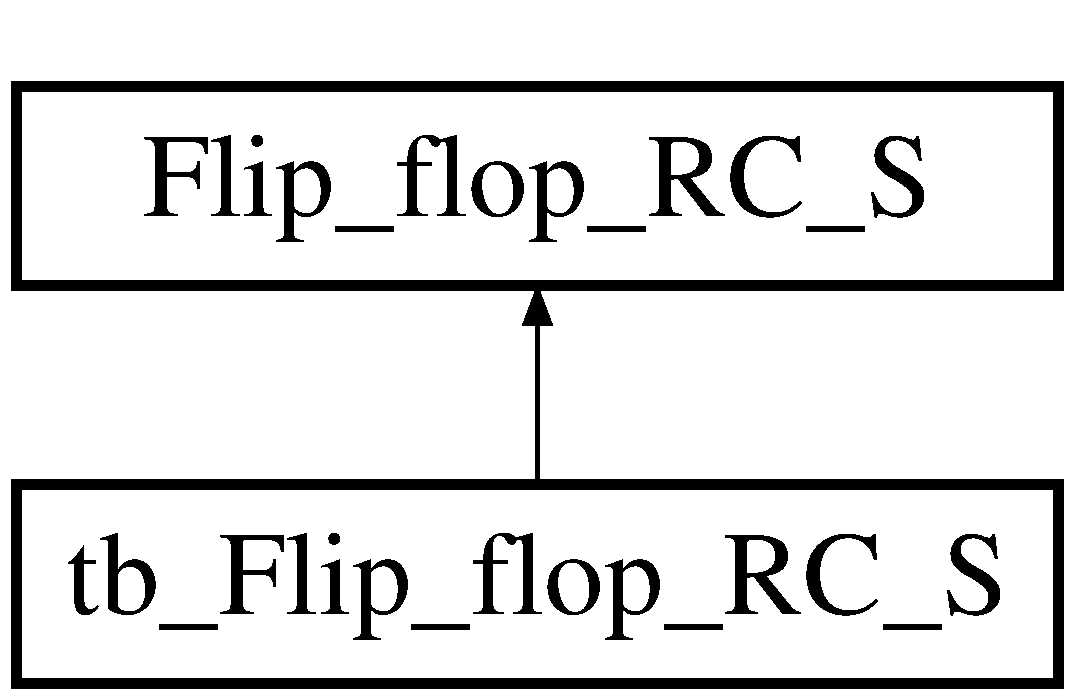
\includegraphics[height=2.000000cm]{class_flip__flop___r_c___s}
\end{center}
\end{figure}
\subsection*{Entities}
\begin{DoxyCompactItemize}
\item 
\hyperlink{class_flip__flop___r_c___s_1_1_behavioral}{Behavioral} architecture
\begin{DoxyCompactList}\small\item\em Architecture definition of the \hyperlink{class_flip__flop___r_c___s}{Flip\+\_\+flop\+\_\+\+R\+C\+\_\+S}. \end{DoxyCompactList}\end{DoxyCompactItemize}
\subsection*{Libraries}
 \begin{DoxyCompactItemize}
\item 
\hyperlink{class_flip__flop___r_c___s_ae4f03c286607f3181e16b9aa12d0c6d4}{I\+E\+EE} \hypertarget{class_flip__flop___r_c___s_ae4f03c286607f3181e16b9aa12d0c6d4}{}\label{class_flip__flop___r_c___s_ae4f03c286607f3181e16b9aa12d0c6d4}

\begin{DoxyCompactList}\small\item\em Use standard library. \end{DoxyCompactList}\end{DoxyCompactItemize}
\subsection*{Use Clauses}
 \begin{DoxyCompactItemize}
\item 
\hyperlink{class_flip__flop___r_c___s_aa4b2b25246a821511120e3149b003563}{S\+T\+D\+\_\+\+L\+O\+G\+I\+C\+\_\+1164}   \hypertarget{class_flip__flop___r_c___s_aa4b2b25246a821511120e3149b003563}{}\label{class_flip__flop___r_c___s_aa4b2b25246a821511120e3149b003563}

\begin{DoxyCompactList}\small\item\em Use logic elements. \end{DoxyCompactList}\end{DoxyCompactItemize}
\subsection*{Ports}
 \begin{DoxyCompactItemize}
\item 
\hyperlink{class_flip__flop___r_c___s_a6231b307b7958b6060563aa2a93d345a}{clk}  {\bfseries {\bfseries \textcolor{vhdlchar}{in}\textcolor{vhdlchar}{ }}} {\bfseries \textcolor{vhdlchar}{S\+T\+D\+\_\+\+L\+O\+G\+IC}\textcolor{vhdlchar}{ }} \hypertarget{class_flip__flop___r_c___s_a6231b307b7958b6060563aa2a93d345a}{}\label{class_flip__flop___r_c___s_a6231b307b7958b6060563aa2a93d345a}

\item 
\hyperlink{class_flip__flop___r_c___s_a3313e71ab116de6fc03014f85009a19d}{clk\+\_\+ena}  {\bfseries {\bfseries \textcolor{vhdlchar}{in}\textcolor{vhdlchar}{ }}} {\bfseries \textcolor{vhdlchar}{S\+T\+D\+\_\+\+L\+O\+G\+IC}\textcolor{vhdlchar}{ }} \hypertarget{class_flip__flop___r_c___s_a3313e71ab116de6fc03014f85009a19d}{}\label{class_flip__flop___r_c___s_a3313e71ab116de6fc03014f85009a19d}

\item 
\hyperlink{class_flip__flop___r_c___s_a3495b88db081463071853b171449fc35}{sync\+\_\+rst}  {\bfseries {\bfseries \textcolor{vhdlchar}{in}\textcolor{vhdlchar}{ }}} {\bfseries \textcolor{vhdlchar}{S\+T\+D\+\_\+\+L\+O\+G\+IC}\textcolor{vhdlchar}{ }} \hypertarget{class_flip__flop___r_c___s_a3495b88db081463071853b171449fc35}{}\label{class_flip__flop___r_c___s_a3495b88db081463071853b171449fc35}

\item 
\hyperlink{class_flip__flop___r_c___s_a33df59ec6762ee2d16c047ef7f6bf8dd}{uc\+\_\+clear}  {\bfseries {\bfseries \textcolor{vhdlchar}{in}\textcolor{vhdlchar}{ }}} {\bfseries \textcolor{vhdlchar}{S\+T\+D\+\_\+\+L\+O\+G\+IC}\textcolor{vhdlchar}{ }} \hypertarget{class_flip__flop___r_c___s_a33df59ec6762ee2d16c047ef7f6bf8dd}{}\label{class_flip__flop___r_c___s_a33df59ec6762ee2d16c047ef7f6bf8dd}

\item 
\hyperlink{class_flip__flop___r_c___s_aba6d2ffd6b2f4f224611e13d51ad39d3}{i2c\+\_\+set}  {\bfseries {\bfseries \textcolor{vhdlchar}{in}\textcolor{vhdlchar}{ }}} {\bfseries \textcolor{vhdlchar}{S\+T\+D\+\_\+\+L\+O\+G\+IC}\textcolor{vhdlchar}{ }} \hypertarget{class_flip__flop___r_c___s_aba6d2ffd6b2f4f224611e13d51ad39d3}{}\label{class_flip__flop___r_c___s_aba6d2ffd6b2f4f224611e13d51ad39d3}

\item 
\hyperlink{class_flip__flop___r_c___s_ac2686f9ae656723c8104446aba446f46}{uc\+\_\+read}  {\bfseries {\bfseries \textcolor{vhdlchar}{out}\textcolor{vhdlchar}{ }}} {\bfseries \textcolor{vhdlchar}{S\+T\+D\+\_\+\+L\+O\+G\+IC}\textcolor{vhdlchar}{ }} \hypertarget{class_flip__flop___r_c___s_ac2686f9ae656723c8104446aba446f46}{}\label{class_flip__flop___r_c___s_ac2686f9ae656723c8104446aba446f46}

\end{DoxyCompactItemize}


\subsection{Detailed Description}
\hyperlink{class_flip__flop___r_c___s}{Flip\+\_\+flop\+\_\+\+R\+C\+\_\+S} entity brief description Detailed description of this \hyperlink{class_flip__flop___r_c___s}{Flip\+\_\+flop\+\_\+\+R\+C\+\_\+S} design element. 

The documentation for this class was generated from the following file\+:\begin{DoxyCompactItemize}
\item 
C\+:/\+Users/\+Public/\+Documents/\+Github/\+V\+H\+D\+L/\+Flip\+\_\+flop/\hyperlink{_flip__flop___r_c___s_8vhd}{Flip\+\_\+flop\+\_\+\+R\+C\+\_\+\+S.\+vhd}\end{DoxyCompactItemize}

\hypertarget{classtb___flip__flop___r___w}{}\section{tb\+\_\+\+Flip\+\_\+flop\+\_\+\+R\+\_\+W Entity Reference}
\label{classtb___flip__flop___r___w}\index{tb\+\_\+\+Flip\+\_\+flop\+\_\+\+R\+\_\+W@{tb\+\_\+\+Flip\+\_\+flop\+\_\+\+R\+\_\+W}}
Inheritance diagram for tb\+\_\+\+Flip\+\_\+flop\+\_\+\+R\+\_\+W\+:\begin{figure}[H]
\begin{center}
\leavevmode
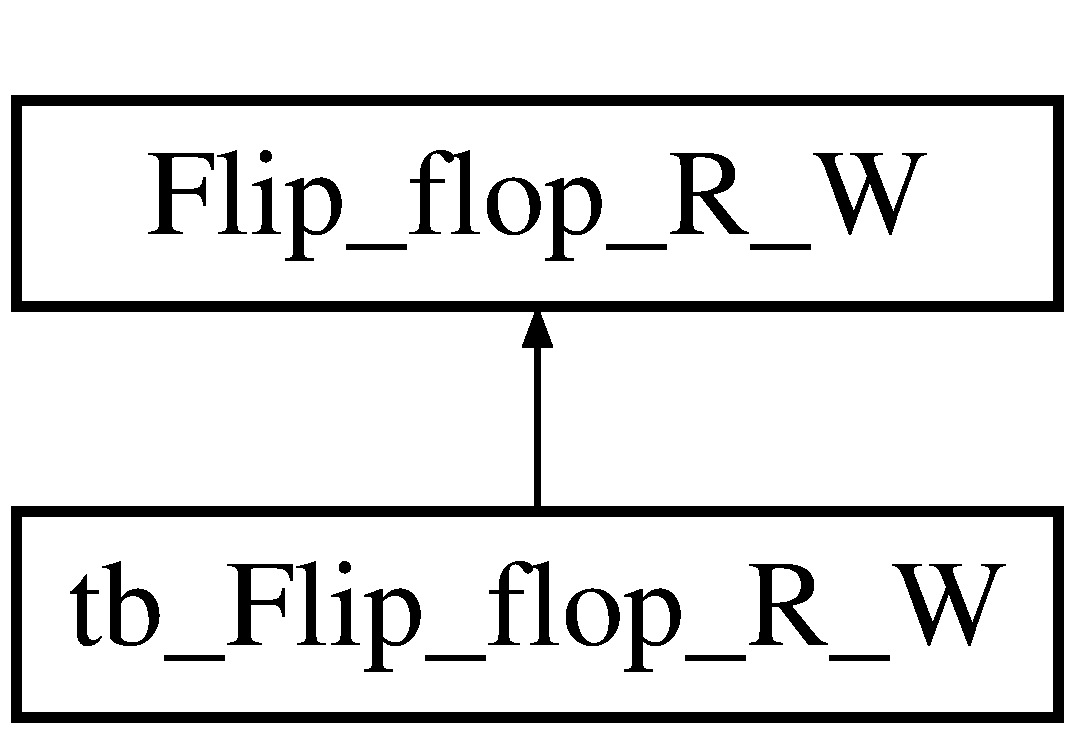
\includegraphics[height=2.000000cm]{classtb___flip__flop___r___w}
\end{center}
\end{figure}
\subsection*{Entities}
\begin{DoxyCompactItemize}
\item 
\hyperlink{classtb___flip__flop___r___w_1_1_behavioral}{Behavioral} architecture
\begin{DoxyCompactList}\small\item\em Architecture definition of the \hyperlink{classtb___flip__flop___r___w}{tb\+\_\+\+Flip\+\_\+flop\+\_\+\+R\+\_\+W}. \end{DoxyCompactList}\end{DoxyCompactItemize}
\subsection*{Libraries}
 \begin{DoxyCompactItemize}
\item 
\hyperlink{classtb___flip__flop___r___w_ae4f03c286607f3181e16b9aa12d0c6d4}{I\+E\+EE} \hypertarget{classtb___flip__flop___r___w_ae4f03c286607f3181e16b9aa12d0c6d4}{}\label{classtb___flip__flop___r___w_ae4f03c286607f3181e16b9aa12d0c6d4}

\begin{DoxyCompactList}\small\item\em Use standard library. \end{DoxyCompactList}\end{DoxyCompactItemize}
\subsection*{Use Clauses}
 \begin{DoxyCompactItemize}
\item 
\hyperlink{classtb___flip__flop___r___w_aa4b2b25246a821511120e3149b003563}{S\+T\+D\+\_\+\+L\+O\+G\+I\+C\+\_\+1164}   \hypertarget{classtb___flip__flop___r___w_aa4b2b25246a821511120e3149b003563}{}\label{classtb___flip__flop___r___w_aa4b2b25246a821511120e3149b003563}

\begin{DoxyCompactList}\small\item\em Use logic elements. \end{DoxyCompactList}\end{DoxyCompactItemize}


The documentation for this class was generated from the following file\+:\begin{DoxyCompactItemize}
\item 
C\+:/\+Users/\+Public/\+Documents/\+Github/\+V\+H\+D\+L/\+Flip\+\_\+flop/\hyperlink{tb___flip__flop___r___w_8vhd}{tb\+\_\+\+Flip\+\_\+flop\+\_\+\+R\+\_\+\+W.\+vhd}\end{DoxyCompactItemize}

\hypertarget{classtb___flip__flop___r_c___s}{}\section{tb\+\_\+\+Flip\+\_\+flop\+\_\+\+R\+C\+\_\+S Entity Reference}
\label{classtb___flip__flop___r_c___s}\index{tb\+\_\+\+Flip\+\_\+flop\+\_\+\+R\+C\+\_\+S@{tb\+\_\+\+Flip\+\_\+flop\+\_\+\+R\+C\+\_\+S}}
Inheritance diagram for tb\+\_\+\+Flip\+\_\+flop\+\_\+\+R\+C\+\_\+S\+:\begin{figure}[H]
\begin{center}
\leavevmode
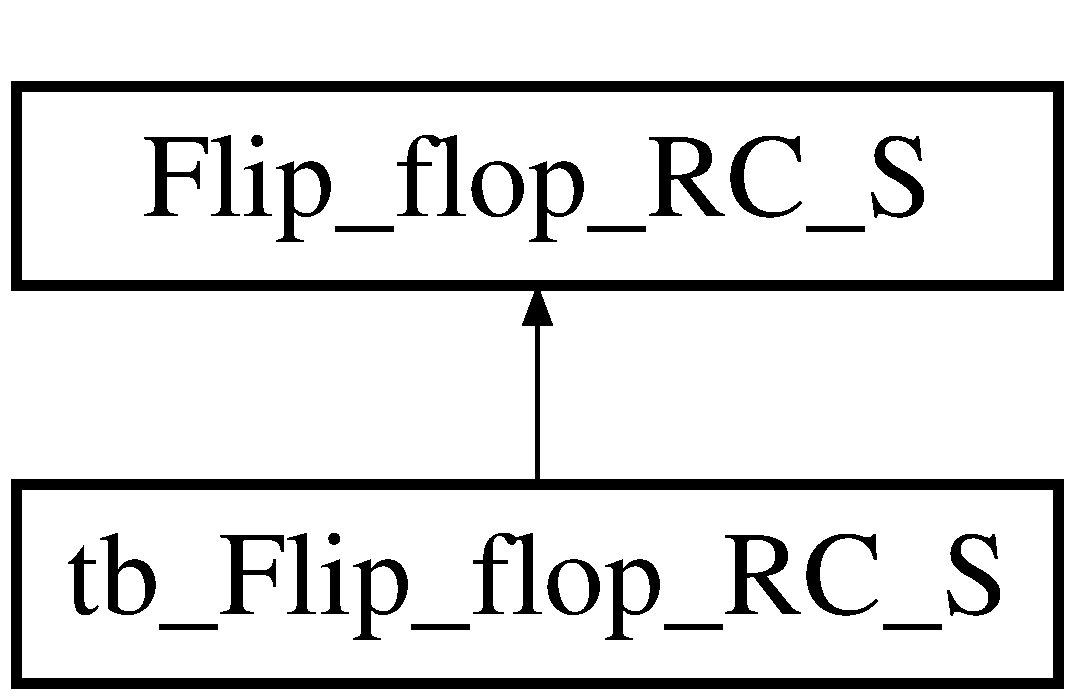
\includegraphics[height=2.000000cm]{classtb___flip__flop___r_c___s}
\end{center}
\end{figure}
\subsection*{Entities}
\begin{DoxyCompactItemize}
\item 
\hyperlink{classtb___flip__flop___r_c___s_1_1_behavioral}{Behavioral} architecture
\begin{DoxyCompactList}\small\item\em Architecture definition of the \hyperlink{classtb___flip__flop___r_c___s}{tb\+\_\+\+Flip\+\_\+flop\+\_\+\+R\+C\+\_\+S}. \end{DoxyCompactList}\end{DoxyCompactItemize}
\subsection*{Libraries}
 \begin{DoxyCompactItemize}
\item 
\hyperlink{classtb___flip__flop___r_c___s_ae4f03c286607f3181e16b9aa12d0c6d4}{I\+E\+EE} \hypertarget{classtb___flip__flop___r_c___s_ae4f03c286607f3181e16b9aa12d0c6d4}{}\label{classtb___flip__flop___r_c___s_ae4f03c286607f3181e16b9aa12d0c6d4}

\begin{DoxyCompactList}\small\item\em Use standard library. \end{DoxyCompactList}\end{DoxyCompactItemize}
\subsection*{Use Clauses}
 \begin{DoxyCompactItemize}
\item 
\hyperlink{classtb___flip__flop___r_c___s_aa4b2b25246a821511120e3149b003563}{S\+T\+D\+\_\+\+L\+O\+G\+I\+C\+\_\+1164}   \hypertarget{classtb___flip__flop___r_c___s_aa4b2b25246a821511120e3149b003563}{}\label{classtb___flip__flop___r_c___s_aa4b2b25246a821511120e3149b003563}

\begin{DoxyCompactList}\small\item\em Use logic elements. \end{DoxyCompactList}\end{DoxyCompactItemize}


The documentation for this class was generated from the following file\+:\begin{DoxyCompactItemize}
\item 
C\+:/\+Users/\+Public/\+Documents/\+Github/\+V\+H\+D\+L/\+Flip\+\_\+flop/\hyperlink{tb___flip__flop___r_c___s_8vhd}{tb\+\_\+\+Flip\+\_\+flop\+\_\+\+R\+C\+\_\+\+S.\+vhd}\end{DoxyCompactItemize}

\chapter{File Documentation}
\hypertarget{_flip__flop___r___w_8vhd}{}\section{C\+:/\+Users/\+Public/\+Documents/\+Github/\+V\+H\+D\+L/\+Flip\+\_\+flop/\+Flip\+\_\+flop\+\_\+\+R\+\_\+W.vhd File Reference}
\label{_flip__flop___r___w_8vhd}\index{C\+:/\+Users/\+Public/\+Documents/\+Github/\+V\+H\+D\+L/\+Flip\+\_\+flop/\+Flip\+\_\+flop\+\_\+\+R\+\_\+\+W.\+vhd@{C\+:/\+Users/\+Public/\+Documents/\+Github/\+V\+H\+D\+L/\+Flip\+\_\+flop/\+Flip\+\_\+flop\+\_\+\+R\+\_\+\+W.\+vhd}}


\hyperlink{class_flip__flop___r___w}{Flip\+\_\+flop\+\_\+\+R\+\_\+W} \+: This entity with synchronization reset is uesd to perform a special port. It could be read by microcontroller and writen by I2C. That means if I2C set \textquotesingle{}i2c\+\_\+write\textquotesingle{} on one, it would put the data of \textquotesingle{}i2c\+\_\+data\+\_\+in\textquotesingle{} into the output \textquotesingle{}uc\+\_\+read\textquotesingle{}. It could be one or zero.\+It just likes its write fonction. Then we can use its output as the input of microcontroller. It likes read by microcontroller.  


\subsection*{Entities}
\begin{DoxyCompactItemize}
\item 
\hyperlink{class_flip__flop___r___w}{Flip\+\_\+flop\+\_\+\+R\+\_\+W} entity
\item 
\hyperlink{class_flip__flop___r___w_1_1_behavioral}{Behavioral} architecture
\begin{DoxyCompactList}\small\item\em Architecture definition of the \hyperlink{class_flip__flop___r___w}{Flip\+\_\+flop\+\_\+\+R\+\_\+W}. \end{DoxyCompactList}\end{DoxyCompactItemize}


\subsection{Detailed Description}
\hyperlink{class_flip__flop___r___w}{Flip\+\_\+flop\+\_\+\+R\+\_\+W} \+: This entity with synchronization reset is uesd to perform a special port. It could be read by microcontroller and writen by I2C. That means if I2C set \textquotesingle{}i2c\+\_\+write\textquotesingle{} on one, it would put the data of \textquotesingle{}i2c\+\_\+data\+\_\+in\textquotesingle{} into the output \textquotesingle{}uc\+\_\+read\textquotesingle{}. It could be one or zero.\+It just likes its write fonction. Then we can use its output as the input of microcontroller. It likes read by microcontroller. 


\hypertarget{_flip__flop___r_c___s_8vhd}{}\section{C\+:/\+Users/\+Public/\+Documents/\+Github/\+V\+H\+D\+L/\+Flip\+\_\+flop/\+Flip\+\_\+flop\+\_\+\+R\+C\+\_\+S.vhd File Reference}
\label{_flip__flop___r_c___s_8vhd}\index{C\+:/\+Users/\+Public/\+Documents/\+Github/\+V\+H\+D\+L/\+Flip\+\_\+flop/\+Flip\+\_\+flop\+\_\+\+R\+C\+\_\+\+S.\+vhd@{C\+:/\+Users/\+Public/\+Documents/\+Github/\+V\+H\+D\+L/\+Flip\+\_\+flop/\+Flip\+\_\+flop\+\_\+\+R\+C\+\_\+\+S.\+vhd}}


\hyperlink{class_flip__flop___r_c___s}{Flip\+\_\+flop\+\_\+\+R\+C\+\_\+S} \+: This entity with synchronization reset is uesd to perform a special port. It could be read or cleared by microcontroller and writen by I2C. That means if microcontroller set \textquotesingle{}uc\+\_\+clear\textquotesingle{} on one, it would set the output on zero. If I2C set \textquotesingle{}i2c\+\_\+set\textquotesingle{} on one, it would set the output on one. It just likes its set fonction. Then we can use its output as the input of microcontroller. It likes read by microcontroller.  


\subsection*{Entities}
\begin{DoxyCompactItemize}
\item 
\hyperlink{class_flip__flop___r_c___s}{Flip\+\_\+flop\+\_\+\+R\+C\+\_\+S} entity
\item 
\hyperlink{class_flip__flop___r_c___s_1_1_behavioral}{Behavioral} architecture
\begin{DoxyCompactList}\small\item\em Architecture definition of the \hyperlink{class_flip__flop___r_c___s}{Flip\+\_\+flop\+\_\+\+R\+C\+\_\+S}. \end{DoxyCompactList}\end{DoxyCompactItemize}


\subsection{Detailed Description}
\hyperlink{class_flip__flop___r_c___s}{Flip\+\_\+flop\+\_\+\+R\+C\+\_\+S} \+: This entity with synchronization reset is uesd to perform a special port. It could be read or cleared by microcontroller and writen by I2C. That means if microcontroller set \textquotesingle{}uc\+\_\+clear\textquotesingle{} on one, it would set the output on zero. If I2C set \textquotesingle{}i2c\+\_\+set\textquotesingle{} on one, it would set the output on one. It just likes its set fonction. Then we can use its output as the input of microcontroller. It likes read by microcontroller. 


\hypertarget{tb___flip__flop___r___w_8vhd}{}\section{C\+:/\+Users/\+Public/\+Documents/\+Github/\+V\+H\+D\+L/\+Flip\+\_\+flop/tb\+\_\+\+Flip\+\_\+flop\+\_\+\+R\+\_\+W.vhd File Reference}
\label{tb___flip__flop___r___w_8vhd}\index{C\+:/\+Users/\+Public/\+Documents/\+Github/\+V\+H\+D\+L/\+Flip\+\_\+flop/tb\+\_\+\+Flip\+\_\+flop\+\_\+\+R\+\_\+\+W.\+vhd@{C\+:/\+Users/\+Public/\+Documents/\+Github/\+V\+H\+D\+L/\+Flip\+\_\+flop/tb\+\_\+\+Flip\+\_\+flop\+\_\+\+R\+\_\+\+W.\+vhd}}


\hyperlink{classtb___flip__flop___r___w}{tb\+\_\+\+Flip\+\_\+flop\+\_\+\+R\+\_\+W} \+:testbench for the entity flip\+\_\+flop\+\_\+r\+\_\+w  


\subsection*{Entities}
\begin{DoxyCompactItemize}
\item 
\hyperlink{classtb___flip__flop___r___w}{tb\+\_\+\+Flip\+\_\+flop\+\_\+\+R\+\_\+W} entity
\item 
\hyperlink{classtb___flip__flop___r___w_1_1_behavioral}{Behavioral} architecture
\begin{DoxyCompactList}\small\item\em Architecture definition of the \hyperlink{classtb___flip__flop___r___w}{tb\+\_\+\+Flip\+\_\+flop\+\_\+\+R\+\_\+W}. \end{DoxyCompactList}\end{DoxyCompactItemize}


\subsection{Detailed Description}
\hyperlink{classtb___flip__flop___r___w}{tb\+\_\+\+Flip\+\_\+flop\+\_\+\+R\+\_\+W} \+:testbench for the entity flip\+\_\+flop\+\_\+r\+\_\+w 


\hypertarget{tb___flip__flop___r_c___s_8vhd}{}\section{C\+:/\+Users/\+Public/\+Documents/\+Github/\+V\+H\+D\+L/\+Flip\+\_\+flop/tb\+\_\+\+Flip\+\_\+flop\+\_\+\+R\+C\+\_\+S.vhd File Reference}
\label{tb___flip__flop___r_c___s_8vhd}\index{C\+:/\+Users/\+Public/\+Documents/\+Github/\+V\+H\+D\+L/\+Flip\+\_\+flop/tb\+\_\+\+Flip\+\_\+flop\+\_\+\+R\+C\+\_\+\+S.\+vhd@{C\+:/\+Users/\+Public/\+Documents/\+Github/\+V\+H\+D\+L/\+Flip\+\_\+flop/tb\+\_\+\+Flip\+\_\+flop\+\_\+\+R\+C\+\_\+\+S.\+vhd}}


\hyperlink{classtb___flip__flop___r_c___s}{tb\+\_\+\+Flip\+\_\+flop\+\_\+\+R\+C\+\_\+S} \+:testbench for the entity flip\+\_\+flop\+\_\+rc\+\_\+s  


\subsection*{Entities}
\begin{DoxyCompactItemize}
\item 
\hyperlink{classtb___flip__flop___r_c___s}{tb\+\_\+\+Flip\+\_\+flop\+\_\+\+R\+C\+\_\+S} entity
\item 
\hyperlink{classtb___flip__flop___r_c___s_1_1_behavioral}{Behavioral} architecture
\begin{DoxyCompactList}\small\item\em Architecture definition of the \hyperlink{classtb___flip__flop___r_c___s}{tb\+\_\+\+Flip\+\_\+flop\+\_\+\+R\+C\+\_\+S}. \end{DoxyCompactList}\end{DoxyCompactItemize}


\subsection{Detailed Description}
\hyperlink{classtb___flip__flop___r_c___s}{tb\+\_\+\+Flip\+\_\+flop\+\_\+\+R\+C\+\_\+S} \+:testbench for the entity flip\+\_\+flop\+\_\+rc\+\_\+s 


%--- End generated contents ---

% Index
\backmatter
\newpage
\phantomsection
\clearemptydoublepage
\addcontentsline{toc}{chapter}{Index}
\printindex

\end{document}
